%%%%%%%%%%%%%%%%%%%%%%%%%%%%%%%%%%%%%%%%%%%%%%%%%%%%%%%%%%
%%
%%  LOD-L8.tex
%%  Lecture 8: Local Diffeology, Modeling
%%
%%%%%%%%%%%%%%%%%%%%%%%%%%%%%%%%%%%%%%%%%%%%%%%%%%%%%%%%%%

\chapter*{\S L8. Local Diffeology, Modeling}
\setcounter{footnote}{0}

%%%%%%%%%%%%%%%%%%%%%%%%%%%%%%%%%%%%%%%%%%%%%%%%%%%%%%%%%%
%%
%% MARK: Abstract
%%
%%%%%%%%%%%%%%%%%%%%%%%%%%%%%%%%%%%%%%%%%%%%%%%%%%%%%%%%%%
\begin{abstract}
  In this lecture we shall see how local diffeology builds a new branch of diffeology with the modeling process.
\end{abstract}

%%%%%%%%%%%%%%%%%%%%%%%%%%%%%%%%%%%%%%%%%%%%%%%%%%%%%%%%%%
%%
%% MARK: Introduction
%%
%%%%%%%%%%%%%%%%%%%%%%%%%%%%%%%%%%%%%%%%%%%%%%%%%%%%%%%%%%


%%%%%%%%%%%%%%%%%%%%%%%%%%%%%%%%%%%%%%%%%%%%%%%%%%%%%%%%%%
%%
%% MARK:  Local diffeology
%%
%%%%%%%%%%%%%%%%%%%%%%%%%%%%%%%%%%%%%%%%%%%%%%%%%%%%%%%%%%
\section{Local diffeology}

\begin{Article}{Local smooth maps.}{}
  We have seen what is a local smooth map
  $$%
    f \colon X \supset A \to X',
  $$%
  where $X$ and $X'$ are two diffeological spaces.
  The map $f$ is \emph{local smooth} if for all plots $P \colon U \to X$,
  the following composite is a plot:
  $$%
    f \circ P \colon P^{-1}(A) \to X'
  $$%
  %
  \smuline{Proposition.} {\itshape The composition of local smooth maps is a local smooth map.}

  Note that the composite of two local smooth maps may be empty,
  the empty map is assumed to be smooth.
\end{Article}


\begin{Article}{D-topology.}{}
  We have seen that,
  if $f \colon X \supset A \to X'$ is a local smooth map,
  then for all plots $P \in \cD$ (the diffeology of $X$) the preimage $P^{-1}(A)$ is open (an open subset of $\Domain(P)$).
  We then defined the \emph{D-topology} as the finest topology on $X$ such that the plots are continuous,
  that is,

  \hspace{1em} $\bullet$ A subset $\cO \subset X$ is \emph{D-open} if $P^{-1}(\cO)$ is open for all plots in $X$.

  Thus,
  the local smooth maps from $X$ to $X'$ are the maps $f$ defined on D-open subsets $A$ of $X$ such that restricted to $A$,
  $f\restriction A$ is smooth for the subset diffeology.
\end{Article}

\begin{Article}{Embedded subsets.}{}
  What is interesting with the D-topology,
  which is a perfect byproduct of the diffeology,
  is the definition of \emph{embedded subsets} that results immediately,
  without the introduction of anything else.

  Consider a subset $A \subset X$,
  and $j \colon A \to X$ be the inclusion.
  We have on $A$ the subset diffeology of $X$,
  let us denote it by $\cD_A = j^*(\cD)$,
  with $\cD$ the diffeology of $X$.

  We have also on $X$ the D-topology $\Torus$,
  and on $A$ the D-topology $T_A$ of $\cD_A$.

  But we have also the pullback $j^*(\Torus)$ of the D-topology of $X$ on $A$.

  \uline{Definition.} {\itshape We say that a subset $A \subset X$ is embedded in the diffeological space $X$,
  if the D-topology $T_A$ of the subspace $A$ coincides with the pullback $j^*(\Torus)$ of the D-topology of $X$ on $A$.
  $$%
    T_A = j^*(\Torus) \quad \Leftrightarrow \quad A \text{ is embedded in } X.
  $$%
  }
  In other words,

  \uline{Criterion} The subset $A \subset X$ is embedded if and only if for any D-open subset $\omega \subset A$,
  equipped with the subset diffeology,
  there exists an open subset $\Omega \subset X$,
  of the D-topology of $X$,
  such that $\omega = \Omega \cap A$.
\end{Article}

\begin{Article}{Example: The rational numbers.}{}
  The rational numbers $\QQ \subset \RR$ are discrete but not embedded.
  What is interesting here is that from a pure topological point of view, only embedded subgroups of $\RR$ are regarded as discrete.
  They are all of the form $a\ZZ$,
  for any number $a$.

  In diffeology it is more precise,
  we can have subgroups discrete and embedded,
  they coincide with the discrete subgroups from the topology point of view,
  and the discrete subgroups which are just induced but not embedded.
\end{Article}

\begin{proof}
  We know that $\QQ$ is discrete,
  that is,
  the plots are locally constant.
  Thus,
  any point $q \in \QQ$ is open of the D-topology of the induced diffeology,
  since the pullback of $q$ by a plot is a component of the domain of the plot,
  then open.
  I recall that to be locally constant for a plot means to be constant on the connected components of the domain of the plot.
  Therefore,

  \smuline{Proposition.} {\itshape The D-topology of a discrete diffeological space is discrete.}

  Now,
  the intersection of an open subset of $\RR$ with $\QQ$ is always infinite,
  since $\QQ$ is dense.
  Therefore,
  $\QQ$ is not embedded.
  And we can conclude also that a strict subgroup $\Gamma \subset \RR$,
  which is discrete,
  is embedded if and only if,
  for any element $\gamma \in \Gamma$ there is an interval $\OpenInterval{\gamma-\epsilon, \gamma + \epsilon}$ such that  $\OpenInterval{\gamma-\epsilon, \gamma + \epsilon} \cap \Gamma = \{\gamma\}$.
  Hence there exists a smallest element $0 < a$ in $\Gamma$,
  and therefore $\Gamma = a \ZZ$.
\end{proof}

\begin{Article}{Embeddings.}{}
  Let $A$ and $X$ be two diffeological spaces and $j \colon A \to X$ be a map.
  We say that $j$ is an embedding if
  \begin{enumerate}
    \item $j$ is an induction.
    \item $j(A) \subset X$ is embedded.
  \end{enumerate}
\end{Article}

\begin{Article}{Example: The group $\GL(n,\RR)$.}{}
  Consider the group of linear isomorphisms $\GL(n,\RR) \subset \Diff(\RR^n)$.
  The group of diffeomorphisms is equipped with the functional diffeology of group of diffeomorphisms,
  that is,
  a parametrization $r \mapsto f_r$ in $\Diff(\RR^n)$,
  defined on $U$,
  is smooth if and only if:
  \begin{enumerate}
    \item $(r,x) \mapsto f_r(x)$,
    defined on $U \times \RR^n$ is a plot in $\RR^n$.
    \item $(r,x) \mapsto (f_r)^{-1}(x)$,
    defined on $U \times \RR^n$ is a plot in $\RR^n$.
  \end{enumerate}
  As a subset of $\Diff(\RR^n)$,
  $\GL(n,\RR)$ inherits the functional diffeology.

  On the other hand,
  the group $\GL(n,\RR)$ is the open subset of $\RR^{n \times n}$:
  $$%
    \GL(n,\RR) = \{ (m_{ij})_{i,j = 1}^n \mid m_{ij} \in \RR \text{ and } \det((m_{ij})_{i,j = 1}^n) \neq 0 \}.
  $$%
  %
  \smuline{Proposition.} {\itshape The injection $j \colon \GL(n,\RR) \to \Diff(\RR^n)$ is an embedding.}
\end{Article}

\begin{proof}
  First of all,
  $j$ is injective.

  Let us prove that $j$ is an induction.
  Let $r \mapsto f_r$ be a plot in $\Diff(\RR^n)$ with values in $\GL(n,\RR)$.
  Let $\bme_i$ be the canonical basis of $\RR^n$ and $\bme_i^*$ the dual basis.
  Then,
  the coefficients of $f_r$ are given by $m_{ij}(r) =\bme_i^*(f_r(\bme_j)$.
  They are obviously smooth,
  by definition of the functional diffeology.

  Now,
  let us prove that $j$ is an embedding.
  Consider the open ball $B(\Id_n,\varepsilon)$,
  centered at the identity and of radius $\varepsilon$.
  Let $\Omega_{\varepsilon}$ be the set of all diffeomorphisms defined by
  %
  \begin{displaymath}
    \Omega_{\varepsilon} = \{f \in \Diff(\RR^{n}) \mid \Der(f)(0) \in B(\Id_n,\varepsilon) \},
  \end{displaymath}
  %
  where $\Der(f)(0)$ is the tangent linear map of $f$ at the point $0$.
  Now,
  let us prove the following:

  (a) The set $\Omega_{\varepsilon}$ is open
  for the D-topology of $\Diff(\RR^{n})$.

  Let $P : U \rightarrow \Diff(\RR^{n})$ be a plot,
  that is,
  $[(r,x)\mapsto P(r)(x)]\in \Cinfty(U \times \RR^{n},\RR^{n})$.
  The pullback of $\Omega_{\varepsilon}$ by $P$ is the set of $r \in U$ such that the tangent map $\Der(P(r))(0)$ is in the ball $B(\Id_n, \varepsilon)$,
  formally,
  $$%
    P^{-1}(\Omega_{\varepsilon}) = \{ r\in U \mid \Der(P(r))(0) \in B(\Id_n, \varepsilon) \}.
  $$%
  Considering $P$ as a smooth map
  defined on
  $U \times \RR^{n}$,
  $\Der(P(r))(0)$ is the partial derivative of $P$,
  with respect to the second variable,
  computed at the point $x=0$.
  The map $[r \mapsto \Der(P(r))(0)]$ is then continuous,
  by definition of smoothness.
  Hence,
  the pullback of $\Omega_{\varepsilon}$ by this map is open.
  Because the imprint of this open set on $\GL(n,\RR)$ is exactly the ball $B(\Id_n, \varepsilon)$,
  we deduce that any open ball of $\GL(n,\RR)$ centered at $\Id_n$ is the imprint of a D-open set of $\Diff(\RR^{n})$.

  (b) Every open of $\GL(n,\RR)$ is the imprint of a D-open set of $\Diff(\RR^n)$.

  By using the group operation on $\GL(n,\RR)$ and since any open set of $\GL(n,\RR)$ is a union of open balls,
  every open subset of $\GL(n,\RR)$ is the imprint of some D-open subset of $\Diff(\RR^n)$.
  Therefore,
  $\GL(n,\RR)$ is embedded in $\Diff(\RR^{n})$.
\end{proof}

\begin{Article}{Functional diffeology on local smooth maps.}{}
  Let $X$ and $X'$ be two diffeological spaces.
  Let $\Cinfty_\loc(X,X')$ be the set of local smooth maps from $X$ to $X'$.
  The evaluation map is defined on
  $$%
    \fF = \{ (f,x) \mid f \in \Cinfty_\loc(X,X') \text{ and } x \in \Domain(f) \}
  $$%
  The evaluation map is,
  as usual,
  $$%
    \Eval \colon \Cinfty_\loc(X,X') \times X \supset \fF \to X' \quad \text{with} \quad \Eval(f,x) = f(x).
  $$%
  %
  \smuline{Proposition.} {\itshape There exists a coarsest diffeology on $\Cinfty_\loc(X,X')$ such that the evaluation map is local smooth.}

  That is,
  $\fF$ is a D-open subset of $\Cinfty_\loc(X,X') \times X$,
  and the map $\Eval$ is smooth with $\fF$ equipped with the subset diffeology.

  A parametrization $r \mapsto f_r$ in $\Cinfty_\loc(X,X')$,
  defined on $U$,
  is a plot if and only if the map
  $$%
    \psi \colon (r,x) \mapsto f_r(x)
  $$%
  defined on
  \begin{align*}
    P^*(\fF) & =  \{ (r,f, x) \in U \times X \mid f = f_r \text{ and } x \in \Domain(f)\} \\
    & \simeq \{ (r,x) \in U \times X \mid x \in \Domain(f_r)\}
  \end{align*}
  with value in $X'$,
  is local smooth.

  Note that $(r,x) \mapsto f_r(x)$ is the composite $\Eval \circ \pphi$,
  where $\pphi(r,x) = (f_r,x)$.

  $$%
    \begin{tikzcd}[column sep=small,every label/.append style = {font = \small}]
    U \times X \supset P^*(\fF) \arrow[d, swap, "\Proj_1"]  \arrow[r, "\pphi"] & \fF \arrow[r, "\Eval"] \arrow[d, "\Proj_1"] & X \\
    U  \arrow[r, "P"] & \Cinfty_\loc(X,X')  &
    \end{tikzcd}
  $$%
\end{Article}

\begin{Article}{Example: Functional diffeology on D-open sets.}{}
  Let $X$ be a diffeological space.
  We get a diffeology on the set of D-open subsets of $X$ as follows:
  consider a family of D-open subsets defined on some Euclidean domain $U$:
  $$%
    r \mapsto \cO(r),
  $$%
  we can decide that the family is a plot in the set of D-open subsets of $X$ if the map
  $$%
    r \mapsto   \Id_{\cO(r)}
  $$%
  is a plot in the space of local smooth maps.
  That is,
  if the subset
  $$%
    \cU = \{(r,x) \in U \times X \mid x \in \cO(r) \}
  $$%
  is a D-open subset on $U \times X$.

  \uline{For example},
  let $r \mapsto I_r$ be a parametrization of open intervals in $\RR$.
  This family is smooth if for all $r_0$ and $x_0 \in \RR$ such that $x_0 \in I_{r_0}$,
  there exists a small ball $B$ centered at $r_0$ and $\epsilon > 0$ such that for all $r \in B$,
  $\OpenInterval{x_0 - \epsilon, x_0 + \epsilon} \subset I_r$.
\end{Article}

%%%%%%%%%%%%%%%%%%%%%%%%%%%%%%%%%%%%%%%%%%%%%%%%%%%%%%%%%%
%%
%% MARK:  Manifolds
%%
%%%%%%%%%%%%%%%%%%%%%%%%%%%%%%%%%%%%%%%%%%%%%%%%%%%%%%%%%%
\section{Manifolds}

We shall present now the classical definition of \emph{manifolds},
and then the diffeology way.

\begin{Article}{Manifolds, the classical way.}{}
  We summarize the basic definitions,
  according to Bourbaki \cite{Bou82},
  but we make the inverse convention,
  made also by some other authors,
  to regard charts defined from real domains to a manifold $M$,
  rather than from subsets of $M$ into real domains.

  ($\clubsuit$) Let $M$ be a nonempty set.
  A {\em chart} of $M$ is a bijection $F$ defined on an $n$-domain $U$ to a subset of $M$.
  The dimension $n$ is a part of the data.
  Let $F : U \to M$ and $F' : U' \to M$ be two charts of $M$.
  The charts $F$ and $F'$ are said to be \emph{compatible} if and only if the following conditions are fulfilled:
  %
  \begin{itemize}
    \item[a)] The sets $F^{-1}(F'(U'))$ and $F'^{-1}(F(U))$ are open.
    \item[b)] The two maps $F'^{-1} \circ F : F^{-1}(F'(U')) \to F'^{-1}(F(U))$ and $F^{-1} \circ F' : F'^{-1}(F(U)) \to F^{-1}(F'(U'))$,
    each one the inverse of the other,
    are either empty or smooth.
    They are called \emph{transition maps}.
  \end{itemize}
  %
  An \emph{atlas} is a set of charts,
  compatible two-by-two,
  such that the union of the values is the whole $M$.
  Two atlases are said to be compatible if their union is still an atlas.
  This relation is an equivalence relation.
  A \emph{structure of manifold} on $M$ is the choice of an equivalence class of atlases or,
  which is equivalent,
  the choice of a \emph{saturated atlas}.
  Once a structure of manifold is chosen for $M$,
  every compatible chart is called a \emph{chart of the manifold}.
\end{Article}

\begin{Article}{Manifolds, the diffeology way.}{}
  Let $X$ be a diffeological space,
  we say that $X$ is an \emph{$n$-manifold} if it is locally diffeomorphic to $\RR^n$ at all points.
  Such local diffeomorphisms from $\RR^n$ to $X$ are called \emph{charts}.
  A generating family of charts is called an \emph{atlas}.

  The Euclidean domains are the first examples of manifolds.
\end{Article}

\begin{Article}{Remark}{}{Where is the difference?}
  The difference between the two definitions gives an advantage to diffeology.
  The difference comes from that in diffeology,
  the set $X$ is \emph{a priori} equipped with a diffeology,
  that is a smooth structure.
  Then,
  the point is to test if the diffeology gives the space a structure of manifold.

  \emph{A contrario},
  with the classical approach,
  the smooth structure is defined \emph{a posteriori}.
  A parametrization $P$ in a manifold $M$ is smooth if the composite by the inverse of the charts is a smooth parametrization of $\RR^n$.

  \uline{Note that} the same set equipped with two different diffeologies may give two different structures of manifolds with different dimensions.
  For example $\RR^2$ can be equipped with its standard diffeology that gives it a structure of a $2$-manifold.
  It can also be equipped with the sum diffeology $X = \sum_{x \in \RR} \RR$ which gives it a structure of $1$-manifold.
\end{Article}

\begin{Article}{Why these definitions give the same category?}{}
  As we said previously,
  given an $n$-manifold $M$ defined by the classical way,
  smooth parametrizations $P$ in $M$ are parametrizations such that $F^{-1} \circ P$ are smooth parametrizations in $\RR^n$.
  We consider the empty parametrization as admissible.
  It is not difficult then to check that the set of these smooth parametrizations define a diffeology for which the charts are local diffeomorphisms.
  Conversely,
  local diffeomorphisms from $\RR^n$ to a diffeological manifold $X$ define on $X$ a structure of manifold,
  the classical way.
  And these two operations are inverse one from each other.
\end{Article}

\begin{Article}{We know already some examples.}{}
  Consider the sphere $\Sph^2 \subset \RR^3$.
  Consider the tangent plane at $N = (0,0,1)$,
  identified with $\RR^2$,
  made of points
  $$%
    X = \Vector{x \\ y \\ 1}
  $$%
  Consider the projection
  $$%
    F \colon X \mapsto m
    \SpacedText{with}
    m = {1 \over \sqrt{x^2 + y^2 +1}} \Vector{x \\ y \\ 1}.
  $$%
  The map $F$ is clearly injective from $\RR^2$ into $\Sph^2$,
  and smooth since $x^2 + y^2 +1$ never vanishes.
  Its inverse is given by
  $$%
    F^{-1} \colon m \mapsto X
    \SpacedText{with}
    X  = \Vector{ x = x'/z'  \\ y = y'/z' \\ z = 1}
    \SpacedText{and}
    m = \Vector{x' \\ y' \\ z'}.
  $$%
  We see here that necessarily $z' \neq 0$ and then $F^{-1}$ is smooth.
  So,
  we got a local diffeomorphism $F$,
  around the North Pole $N$.
  Then,
  we use the transitive action of $\SO(3,\RR)$ to get a local diffeomorphism at all points in $\Sph^2$.

  To this example we have already seen the various tori $\Torus^n = \RR^n/\ZZ^n$.
\end{Article}

\begin{Article}{Diffeological manifolds.}{}
  In diffeology we extend the definition of manifolds.
  A \emph{diffeological manifold} is a diffeological space locally diffeomorphic to a diffeological vector space at all points.

  A \emph{diffeology of vector space} is a diffeology on a vector space for which the addition and the multiplication by a scalar are smooth.
\end{Article}

\begin{Article}{Example: The infinite complex projective space.}
  \label{The-infinite-complex-projective-space}
  We have seen the construction of the infinite projective space in \textsection\,\ref{The-Infinite-Sphere-over-the-Infinite-Projective-Space},
  where
  $$%
    \cP_{\CC} = \cH_{\CC}^\star / \CC^\star
  $$%
  is equipped with the fine diffeology.
  We have introduced the maps $F_k$,
  with $k = 1,2,\ldots$
  $$%
    F_k \colon \cH_{\CC} \to \cP_{\CC}
    \SpacedText{with}
    F_k = \Class \circ j_k, \quad k=1, \ldots, \infty.
  $$%
  That is,
  \begin{multline*}
    F_1(Z) = \Class(1,Z)
    \SpacedText{and} \\
    F_k(Z) = \Class(Z_1,\ldots, Z_{k-1}, 1, Z_k,\ldots), \text{ for } k> 1.
    \end{multline*}
  Then:

  (1) For every $k = 1, \ldots, \infty$, $j_k$ is an induction from $\cH_{\CC}$ into $\cH_{\CC}^{\star}$.

  (2) For every $k = 1, \ldots, \infty$, $F_k$ is a local diffeomorphism from $\cH_{\CC}$ to $\cP_{\CC}$.
  Moreover,
  their values cover $\cP_{\CC}$,
  $$%
    \bigcup_{k=1}^\infty \Val(F_k) = \cP_{\CC}.
  $$%
  % Hence,

  \smuline{Proposition.} The diffeological space $\cP_{\CC}$ is a diffeological manifold modeled on $\cH_{\CC}$,
  for which the family $\{F_k\}_{k=1}^\infty$ is an atlas.

\end{Article} %% The-infinite-complex-projective-space


%%%%%%%%%%%%%%%%%%%%%%%%%%%%%%%%%%%%%%%%%%%%%%%%%%%%%%%%%%
%%
%% MARK:  Manifolds With Boundary
%%
%%%%%%%%%%%%%%%%%%%%%%%%%%%%%%%%%%%%%%%%%%%%%%%%%%%%%%%%%%
\section{Manifolds with boundary}

\begin{Article}{Half-spaces.}{}
  \label{Half-spaces}
  We denote by
  $$%
    \HH_n = \RR^{n-1} \times \LeftClosedInterval{0,\infty}
  $$%
  the \emph{standard half-space} of $\RR^n$.

  We denote by $x=(r,t)$ its points with $r \in \RR^{n-1}$ and $t \in [0,+\infty[$.

  We denote by $\partial \HH_n$ its boundary $\RR^{n-1} \times \{0\}$.
  The subset diffeology of $\HH_n$,
  inherited from $\RR^n$,
  is made of all the smooth parametrizations $P : U \to \RR^n$ such that $P_n(r) \geq 0$ for all $r \in U$,
  $P_n(r)$ being the $n$-th coordinate of $P(r)$.
  The D-topology of $\HH_n$ is the usual topology defined by its inclusion into $\RR^n$.
\end{Article} %% Half-spaces

\begin{Article}{Smooth real maps from half-spaces.}{}
  \label{Smooth-real-maps-from-half-spaces}
  This is a theorem:
  A map $f \colon \HH_n \to \RR^p$ is smooth for the subset diffeology of $\HH_n$ if and only if there exists an ordinary smooth map $F$,
  defined on an open neighborhood of $\HH_n$,
  such that $f = F \restriction \HH_n$.
  Actually,
  there exists such an $F$ defined on the whole $\RR^n$.

  \uline{Note.} As an immediate corollary,
  any map $f$ defined on $\cC \times [0,\varepsilon[$ to $\RR^p$,
  where $\cC$ is an open cube of $\partial \HH_n$,
  centered at some point $(r,0)$,
  smooth for the subset diffeology,
  is the restriction of a smooth map $F : \cC \times \OpenInterval{-\varepsilon, +\varepsilon} \to \RR^p$.
\end{Article} %% Smooth-real-maps-from-half-spaces

\begin{proof}
  First of all,
  if $f$ is the restriction of a smooth map $F \colon \RR^n \to \RR^p$,
  it is obvious that for every smooth parametrization $P : U \to \HH_n$,
  $f\circ P = F \circ P$ is smooth.
  Conversely,
  let $f_i$ be a coordinate of $f$.
  Let $x =(r,t) \in \RR^{n-1} \times \RR$.
  If $f_i$ is smooth for the subset diffeology,
  then $\pphi_i \colon (r,t) \mapsto f_i(r,t^2)$,
  defined on $\RR^n$,
  is smooth.
  Now, $\pphi_i$ is even in the variable $t$,
  $\pphi_i(r,t) = \pphi_i(r,-t)$.
  Thus,
  according to Hassler Whitney \cite[Theorem 1 and final remark]{Whi43},
  see Figure \ref{fig-Whitney-1} and Figure \ref{fig-Whitney-2},
  there exists a smooth map $F_i : \RR^n  \to \RR$ such that:
  $\pphi_i(r,t) = F_i(r,t^2)$.
  Hence,
  $f_i(r,t) = F_i(r,t)$ for all $r \in \RR^{n-1}$ and all $t \in [0,+\infty[$.
\end{proof}

%%###########
\begin{figure}[htb]
  \centerline{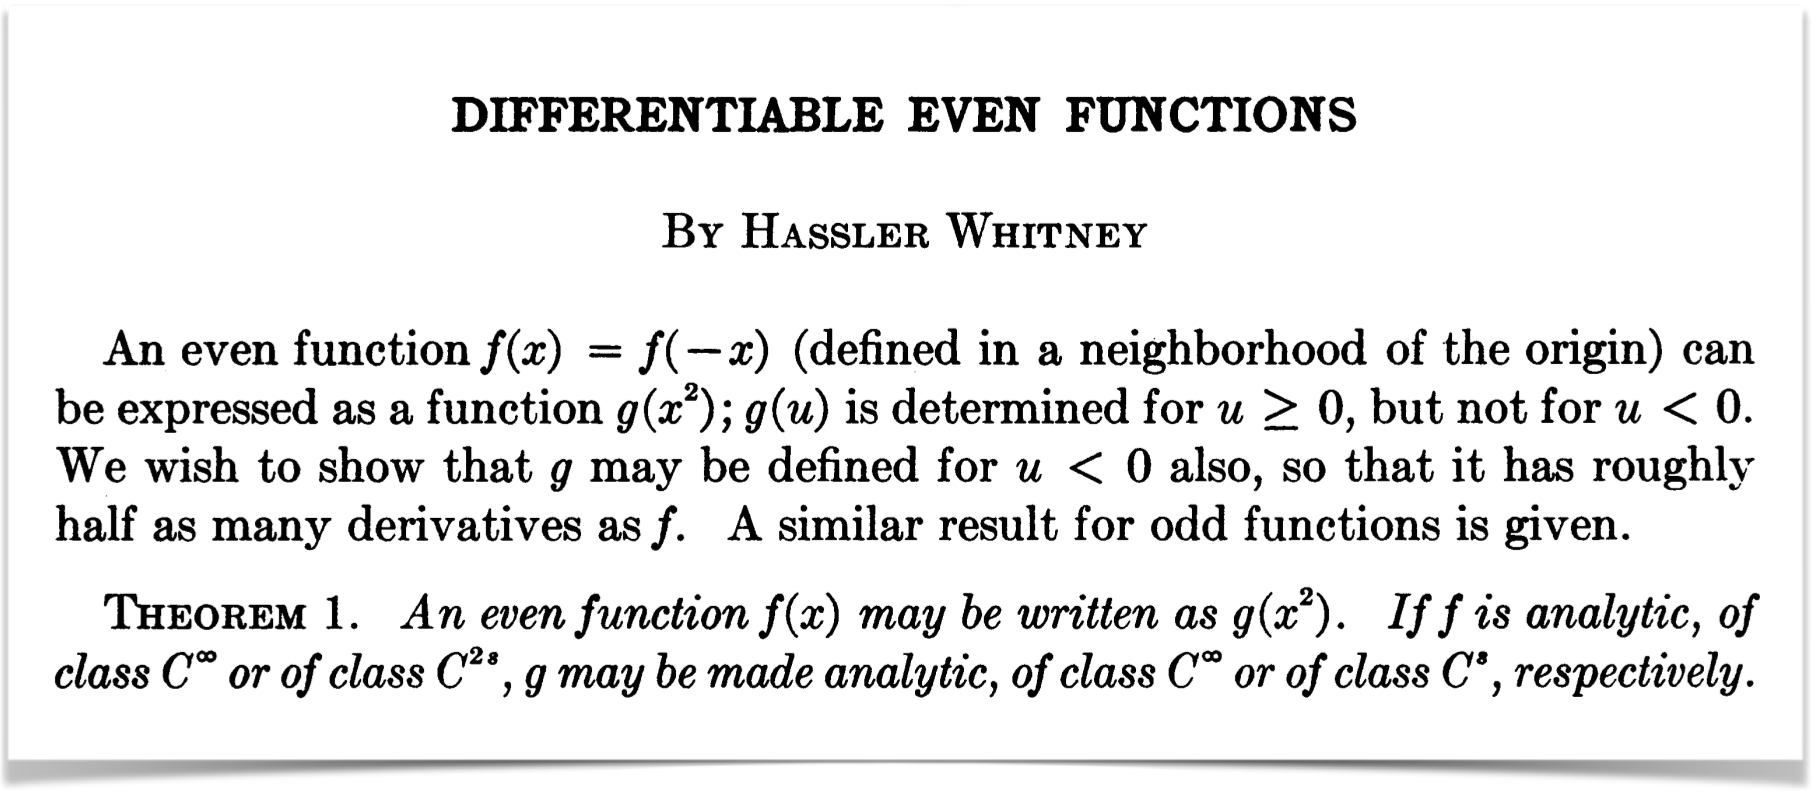
\includegraphics[width=1.0\textwidth]{Figures/Whitney-1.png}}
  \vspace{-10pt}
  \caption{Whitney theorem 1.}
  \label{fig-Whitney-1}
\end{figure}
%%###########

\begin{Article}{Half-spaces local diffeomorphisms.}{}
  \label{Local-diffeomorphisms-of-half-spaces}
  A map $f \colon A \to \HH_n$,
  with $A \subset \HH_n$,
  is a local diffeomorphism for the subset diffeology of $\RR^n$ if and only if
  \begin{enumerate}
    \item $A$ is open in $\HH_n$,
    \item $f$ is injective,
    \item $f(A \cap \partial \HH_n) \subset \partial \HH_n$,
    \item and for all $x \in A$ there exists an open ball $B \subset \RR^n$ centered at $x$,
    and a local diffeomorphism $F \colon B \to \RR^n$ such that $f$ and $F$ coincide on $B \cap \HH_n$.
  \end{enumerate}

  \uline{Note.} This implies in particular,
  that there exists an open neighborhood $\cU$ of $A$ and an \'etale application $g \colon \cU \to \RR^n$ such that $f$ and $g$ coincide on $A$.
\end{Article} %% Local-diffeomorphisms-of-half-spaces

\begin{proof}
  See \cite[\textsection\,4.14]{PIZ13}.
\end{proof}

\begin{Article}{Classical manifolds with boundary.}{}
  \label{Classical-manifolds-with-boundary}
  Manifolds with boundary%
  \linebreak%
  have been precisely defined for example in \cite{GP74} or in \cite{Lee06},
  and others.
  We use here Lee's definition except that,
  for our subject,
  the direction of charts have been reversed.

  \uline{Definition.} A \emph{smooth $n$-manifold with boundary\/} is a topological space $M$,
  together with a family of local homeomorphisms $F_i$ defined on some open sets $U_i$ of the half-space $\HH_n$ to $M$,
  such that the values of the $F_i$ cover $M$ and,
  for any two elements $F_i$ and $F_j$ of the family,
  the transition homeomorphism $F_i^{-1} \circ F_j$,
  defined on $F_i^{-1}(F_i(U_i) \cap F_j(U_j))$ to $F_j^{-1}(F_i(U_i) \cap F_j(U_j))$,
  is the restriction of some smooth map defined on an open neighborhood of $F_i^{-1}(F_i(U_i) \cap F_j(U_j))$.
  The boundary $\partial M$ is the union of the $F_i(U_i \cap \partial \HH_n)$.
  Such a family $\cF$ of homeomorphisms is called an atlas of $M$,
  and its elements are called {\em charts\/}.
  There exists a \emph{maximal atlas} $\cA$ containing $\cF$,
  made with all the local homeomorphisms from $\HH_n$ to $M$,
  such that the transition homeomorphisms with every element of $\cF$ satisfy the condition given just above.
  We say that $\cA$ gives to $M$ its \emph{structure of manifold with boundary}.
\end{Article} %% Classical-manifolds-with-boundary

\begin{Article}{Manifolds with boundary, the diffeology Way.}{}
  \label{Diffeology-of-manifolds-with-boundary}
  Let $X$ be a diffeological space.
  We say that $X$ is an $n$-manifold with boundary if it is locally diffeomorphic to the half-space $\HH_n$ at all points.
  Such local diffeomorphisms are called charts of $X$ and a set of charts that covers $X$ is called an atlas.

  \smuline{Proposition.} This definition is completely equivalent to the classical way above.

  \uline{Note 1.} Here again we shall note that the main difference is that the set $X$ is \emph{a priori} equipped with a diffeology,
  and we just check if its diffeology is a diffeology of manifold with boundary.

  \uline{Note 2.} The diffeology of a classical manifold with boundary $M$ is defined by parametrizations in $M$ such that,
  the composite with the inverse of all charts is smooth.
  That definition creates an equivalence between the classical and the diffeology categories.
\end{Article} %% Diffeology-of-manifolds-with-boundary

%%%%%%%%%%%%%%%%%%%%%%%%%%%%%%%%%%%%%%%%%%%%%%%%%%%%%%%%%%
%%
%% MARK:  Manifolds With Corners
%%
%%%%%%%%%%%%%%%%%%%%%%%%%%%%%%%%%%%%%%%%%%%%%%%%%%%%%%%%%%
\section{Manifolds with corners}

\begin{Article}{Corners.}{}
  \label{Corners}
  We denote by
  $$%
    \KK_n = \LeftClosedInterval{0,\infty}^n
  $$%
  the \emph{standard corner} of $\RR^n$.
  That is,
  the subset
  $$%
    \KK_n = \{ (x_1,\dots,x_n) \mid x_i \geq 0, \forall i = 1 \dots n \}.
  $$%
  The corner $\KK_n$ is equipped with the subset diffeology inherited from $\RR^n$,
  which coincides with the $n$th-power of $\LeftClosedInterval{0,\infty}$.
  The plots are just the smooth parametrizations in $P$ in $\RR^n$ such that,
  for all $i = 1 \dots n$ $P_i(r) \geq 0$.
  The D-topology of $\KK_n$ is the usual topology defined by its inclusion into $\RR^n$.
\end{Article} %% Corners

%%###########
\begin{figure}[htb]
  \centerline{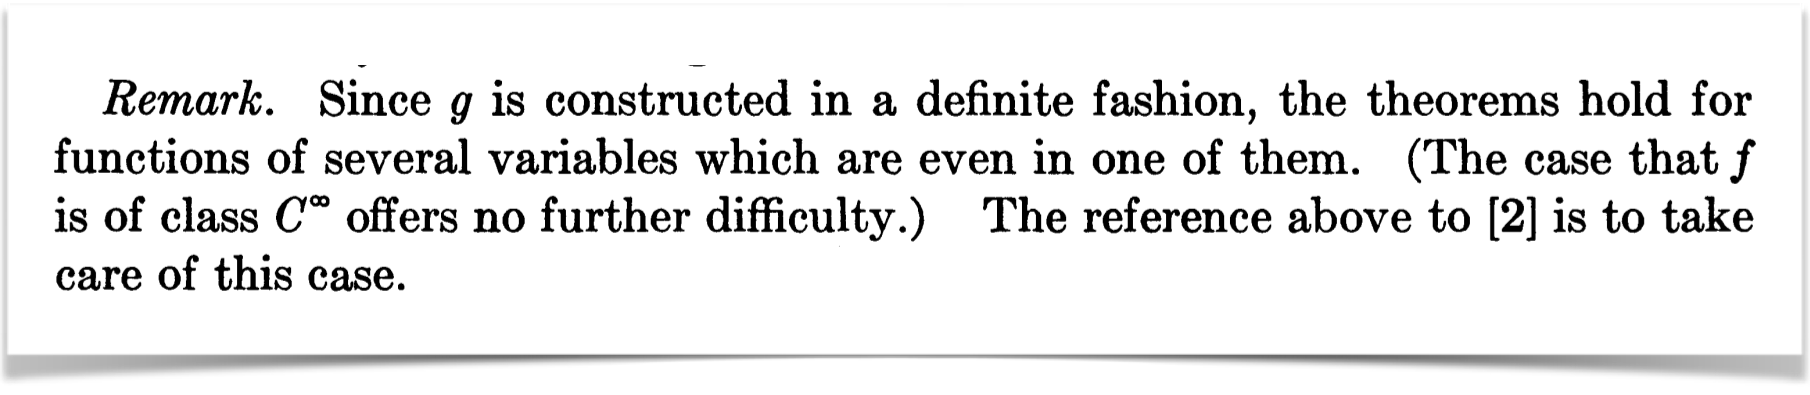
\includegraphics[width=1.0\textwidth]{Figures/Whitney-2.png}}
  \vspace{-10pt}
  \caption{Whitney Last Remark.}
  \label{fig-Whitney-2}
\end{figure}
%%###########
%
\begin{Article}{Local smooth maps on corners.}{}
  A map $f \colon \KK_n \to \RR^k$ is smooth for the subset diffeology if and only if,
  it is the restriction of a smooth map defined on an open neighborhood of $\KK^n$.

  What does that mean precisely?

  Let $f \colon \KK_n \to \RR$ be a map such that:
  for every smooth parametrization $P \colon U \to \RR^n$ taking its values in $\KK_n$,
  $f \circ P$ is smooth.
  Then,
  $f$ is the restriction of a smooth map $F$ defined on some open neighborhood of $\KK_n$.

  What does that say?

  That says that a heuristic consisting of defining a smooth map from the corner $\KK_n$ to $\RR$,
  as the restriction of a smooth map defined on an open neighborhood of $\KK_n$,
  can be avoided by using the diffeology framework.
  Assuming $f$ to be smooth for the subset diffeology does the work,
  and moreover conceptually.
\end{Article}

\begin{proof}
  The proof is a recurrence on the same theorem above for half-spaces,
  see \cite{GIZ19}.
\end{proof}

\begin{Article}{Local diffeomorphisms of corners.}{}
  A local diffeomorphism $f$ from $\KK_n$ into itself is the restriction of an \'etale map defined on some open neighborhood of its domain of definition.
\end{Article}

\begin{Article}{Classical manifolds with corners.}{}
  Let $M$ be a paracompact Hausdorff topological space.
  An $n$-chart with corners for $M$ is a pair $(U,\pphi)$,
  where $U$ is an open subset of $\KK^n$,
  and $\pphi$ is a homeomorphism from $U$ to an open subset of $M$.
  Two charts with corners $(U,\pphi)$ and $(V,\psi)$ are said to be smoothly compatible if the composite map $\psi^{-1} \circ \pphi \colon \pphi^{-1}(\psi(V)) \to \psi^{-1}(\pphi(U))$ is a diffeomorphism,
  in the sense that it admits a smooth extension to an open set in $\RR^n$.
  An $n$-atlas with corners for $M$ is a pairwise compatible family of n-charts with corners covering $M$.
  A maximal atlas is an atlas which is not a proper subset of any other atlas.
  An $n$-manifold with corners is a paracompact Hausdorff topological space $M$ equipped with a maximal $n$-atlas with corners.
\end{Article}

\begin{Article}{Diffeological manifolds with corners.}{}
  A diffeological space $X$ is an $n$-manifold with corners if and only if it is locally diffeomorphic to $\KK_n$ at all points.
\end{Article}

\vfill
\centerline{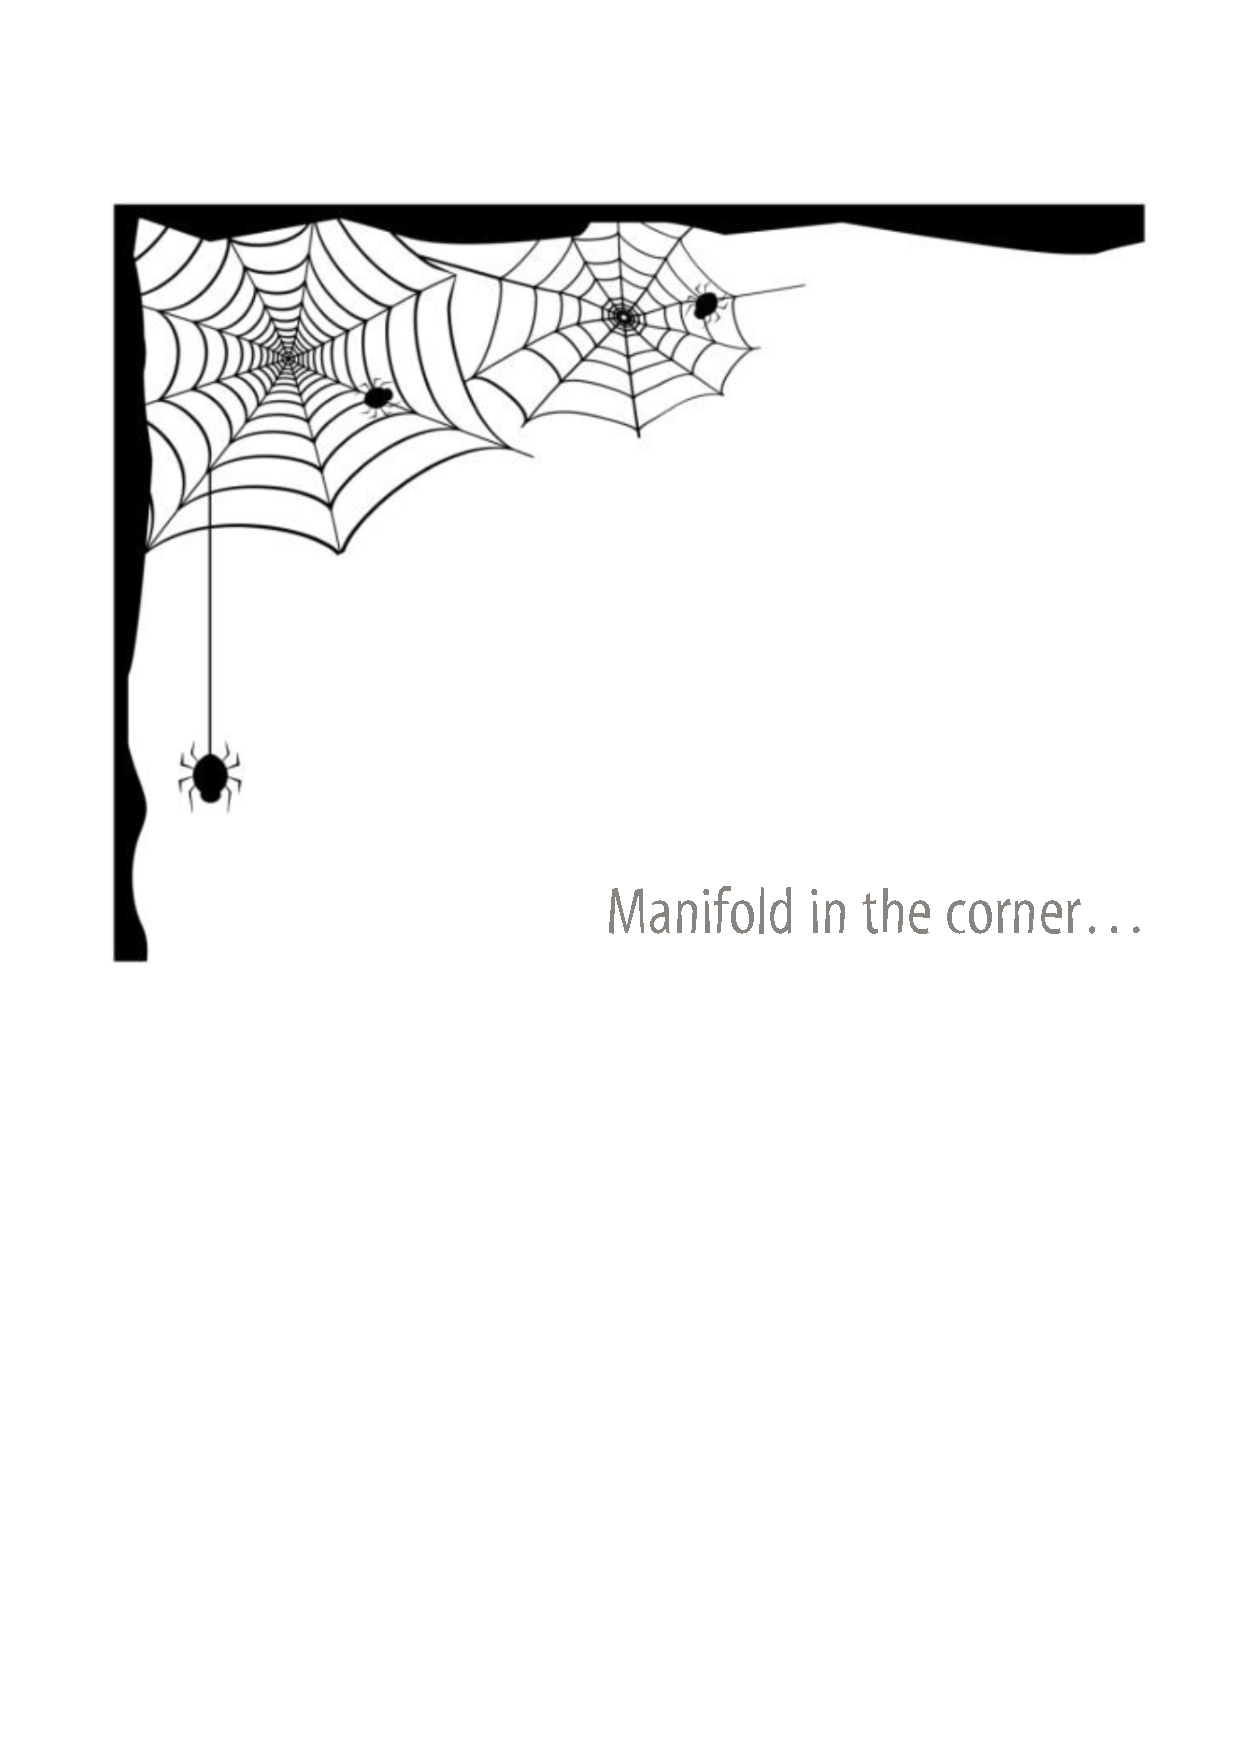
\includegraphics[width=.5\textwidth]{Figures/Manifold-in-the-corner.pdf}}
